%%%%%%%%%%%%%%%%%%%%%%%%%%%%%%%%%%%%%%%%%%%%%%%%%%%%%%%%%%%%%%%%%%%%%%%%%%%%%%%%%%%%%%%%%%%%%%%%
%%%%% Fate African forests

%%%%%%%%%%%%%%%%%% Preambule %%%%%%%%%%%%%%%%%%%%%%%%%%%%%%%%%%

\documentclass[slidetop,10pt,dvipsnames,leqno,fleqn]{beamer} % dvipsnames for choosing colors

%%%%%%%%%%%%%%
%%%%% Packages
%%%%%%%%%%%%%%

%\usepackage{pslatex} % to see correctly a .pdf file on the computer screen
\usepackage{pgf}
%\usepackage[svgnames]{xcolor}
\usepackage{xcolor}
\usepackage{graphicx}
\usepackage{amssymb} %symbole de maths
\usepackage{amsmath} %idem
\usepackage[utf8]{inputenc}
%\usepackage{fancyvrb} %give size to verbatim
%\usepackage{hyperref}
\usepackage[english,francais]{babel}
%\definecolor{vertmoyen}{RGB}{51,110,23} % vert moyen
\xdefinecolor{green}{named}{OliveGreen}
\usecolortheme[named=green]{structure}
\usepackage{tabularx} % varier la largeur du tableau
\usepackage{layout}
\usepackage{longtable}
\setlength{\LTleft}{-5cm plus 1 fill}
\setlength{\LTright}{-5cm plus 1 fill}
\usepackage{booktabs}
%\usepackage{colortabs} % can't be found
\usepackage{xcolor,colortbl} %% color text and table rows
\usepackage{arydshln} %% dashlines for tabular
\newcommand{\logit}{\text{logit}}
\newcommand{\p}{\text{p}}
\newcommand{\bs}[1]{\boldsymbol{#1}}
\newcommand{\R}{\textnormal{\sffamily\bfseries R}}
\newcommand{\pkg}[1]{{\fontseries{b}\selectfont #1}}
\newcolumntype{C}[1]{>{\centering\arraybackslash}m{#1}}
\newcolumntype{R}[1]{>{\raggedleft\arraybackslash}m{#1}}
\newcolumntype{L}[1]{>{\raggedright\arraybackslash}m{#1}}
\usepackage{ulem} % Texte barré, souligné
%% Natbib is a popular style for formatting references.
%\usepackage{natbib} %doesn't work with beamer

\title[Modelling deforestation]{Accounting for spatial autocorrelation in deforestation modelling (and forecasting)}
%\subtitle{} 

\date{}

% Theme
\usetheme{Dresden}
% \usetheme{Copenhagen}
% \usetheme{Frankfurt}
% \usetheme{Berlin}
% \usetheme{Madrid}
% \usetheme{Montpellier}
% \usetheme{Singapore}
% \usetheme{Antibes}
\useinnertheme{rounded}

% Logo
\newif\ifplacelogo % create a new conditional
\logo{\ifplacelogo\includegraphics[width=2.5cm]{./Figures/Logo-JRC.jpg}\fi} % replace with your own command

% %Page number
% \addtobeamertemplate{footline}{
%   \hspace{0.15cm} \insertframenumber \vspace{0.15cm}
% }

% %Call table of contents at the beginning of each section
% \AtBeginSection[]{
% \placelogotrue
%   \begin{frame}
%     \framesubtitle{Plan}
%     \begin{columns}[c]
%       \begin{column}{0.5\textwidth}
%         \tableofcontents[sections={1-2},currentsection]
%       \end{column}
%       \begin{column}{0.5\textwidth}
%         \tableofcontents[sections={3-4},currentsection]
%       \end{column}
%     \end{columns}
%   \end{frame}
% \placelogofalse
% }

% \AtBeginSubsection[]{
%   \begin{frame}
%     \framesubtitle{Plan}
%     \begin{columns}[c]
%       \begin{column}{0.5\textwidth}
%         \tableofcontents[sections={1-2},currentsection,currentsubsection]
%       \end{column}
%       \begin{column}{0.5\textwidth}
%         \tableofcontents[sections={3-4},currentsection,currentsubsection]
%       \end{column}
%     \end{columns}
%   \end{frame}
% }

%%%%%%%%%%%%%%%%%% \End Preambule %%%%%%%%%%%%%%%%%%%%%%%%%%%%%%

\begin{document}

% Title page
{
  \setbeamertemplate{navigation symbols}{}

  % Title page
  \begin{frame}[plain]
    \begin{center}
      \small{\textbf{ISEC -- 5 July 2018}}
    \end{center}
    \vspace{-0.5cm}
    \titlepage % Presentation first page
    \vspace{-2.5cm}
    \begin{center}
      \includegraphics[width=10cm]{./Figures/Banniere.png}
    \end{center}
    \begin{center}

      {\footnotesize
        \begin{tabular}{c}
          Ghislain Vieilledent$^{1,2}$ and Frédéric Achard$^{1}$ \\
        \end{tabular}
      }

      \vspace{0.25cm}

      {\scriptsize
        \begin{tabular}{c}
          $[1]$ \textbf{EU Joint Research Center}, Ispra, ITALY\\
          $[2]$ \textbf{Cirad}, Montpellier, FRANCE \\
        \end{tabular}
      }

      \vspace{0.25cm}

      \begin{tabular}{C{2cm}C{1cm}C{2cm}}
        \includegraphics[height=0.7cm]{./Figures/Logo-JRC.jpg} &
        ~ &
        \includegraphics[height=0.7cm]{./Figures/Logo-Cirad.png}\\
      \end{tabular}

    \end{center}
    
  \end{frame}

}

% %%%%%%%%%%%%%%%%%%%%%%%%%%%%%%%%%%%%%%%%%%%%%%%%%%%%%%%%%%%%%%%%

% \placelogotrue
% \begin{frame}
%   \framesubtitle{Outline}
%   \begin{columns}[c]
%     \begin{column}{0.5\textwidth}
%       \tableofcontents[sections={1-2}]
%     \end{column}
%     \begin{column}{0.5\textwidth}
%       \tableofcontents[sections={3-4}]
%     \end{column}
%   \end{columns}
% \end{frame}
% \placelogofalse

%%///////////////////////////////////////
\section{Introduction}

\begin{frame}
  \frametitle{Motivation}
  \framesubtitle{}
  \begin{columns}[c]
    \begin{column}{0.5\textwidth}
      \begin{block}{Consequences of deforestation}
        \begin{itemize}
        \item Biodiversity loss
        \item Carbon emissions and climate change
        \end{itemize}
      \end{block}
      \begin{block}{Modelling deforestation}
        \begin{itemize}
        \item Scenarios of biodiversity (IPBES) and CO$_2$ emissions (IPCC)
        \item Anticipate and take action (ex. policies)
        \end{itemize}
      \end{block}
    \end{column}
    \begin{column}{0.5\textwidth}
      \centering \includegraphics[width=5cm]{./Figures/Thuiller2007-Nature.png}\\
      {\small Thuiller 2007, \textit{Nature}}
    \end{column}
  \end{columns}
\end{frame}

\begin{frame}
  \frametitle{Focus}
  \framesubtitle{}
  \begin{columns}[c]
    \begin{column}{0.5\textwidth}
      \begin{block}{Location of deforestation}
        \begin{itemize}
        \item \sout{How much deforestation? (deforestation rates)}
        \item Where deforestation occurs preferentially?
        \item Biodiversity and carbon stock vary spatially
        \end{itemize}
      \end{block}    
    \end{column}
    \begin{column}{0.5\textwidth}
      \centering \includegraphics[width=4cm]{./Figures/Vieilledent2016-JoE.jpg}\\
      {\small Vieilledent et al. 2016, \textit{J. of Ecol.}}
    \end{column}
  \end{columns}
\end{frame}

\begin{frame}
  \frametitle{State of art}
  \framesubtitle{}
  \begin{block}{Model}
    \begin{itemize}
    \item $Y_i \in \{0, 1\}$
    \item $Y_i \sim \mathcal{B}ernoulli(\theta_i)$
    \item $\logit(\theta_i) = f(\text{spatial factors}_i)$
    \end{itemize}
  \end{block}
  \begin{block}{Spatial factors}
    \begin{itemize}
    \item \textbf{Landscape}: distance to forest edge
    \item \textbf{Accessibility}: altitude, slope, distance to road, town
    \item \textbf{Land-policy}: protected area network
    \end{itemize}
  \end{block}
\end{frame}

\begin{frame}
  \frametitle{Research gap}
  \framesubtitle{}
  \begin{block}{Unmeasured factors}
    \begin{itemize}
    \item Many other explicative spatial factors
    \item Population density, soil, geographical barriers, controls... 
    \item Some \textbf{not measured}, some \textbf{unmeasurable}
    \end{itemize}
  \end{block}
  \begin{block}{Proposed model}
    \begin{itemize}
    \item $\logit(\theta_{ij}) = f(\text{spatial factors}_i) + \rho_j$
    \item Spatial random effects $\rho_j$ to account for unmeasured factors
    \end{itemize}
  \end{block}
\end{frame}

\begin{frame}
  \frametitle{Objective}
  \framesubtitle{}
  \begin{block}{Model comparison}
    \begin{itemize}
    \item Model 1: $\logit(\theta_{ij}) = f(\text{spatial factors}_i)$
    \item Model 2: $\logit(\theta_{ij}) = f(\text{spatial factors}_i) + \rho_j$
    \end{itemize}
  \end{block}
  \begin{block}{Challenge}
    \begin{itemize}
    \item Use the model for forecasting (not only for inference)
    \item On large spatial scale
    \end{itemize}
  \end{block}
\end{frame}

%%///////////////////////////////////////
\section{Methods}

\begin{frame}
  \frametitle{Data}
  \framesubtitle{}
  \begin{center}
    \includegraphics[width=\textwidth]{./Figures/deforestation_sambirano.JPG}\\
    Deforestation process in Madagascar. Current rate: 100,000~ha/yr.
  \end{center}
\end{frame}

\begin{frame}
  \frametitle{Data}
  \framesubtitle{}
    \begin{columns}
    \begin{column}{0.45\textwidth}
      \begin{block}{Response variable}
        \begin{itemize}
        \item $Y_i \in \{0, 1\}$
        \item Deforestation in Madagascar on the period 2000-2010
        \item 30~m resolution
        \item 20,000 points $i$ (deforested/non-deforested)  
        \end{itemize}
      \end{block}
    \end{column}
    \begin{column}{0.55\textwidth}
      \centering \includegraphics[width=6cm]{./Figures/fig_fcc.png}\\
      {\small Vieilledent et al. 2018 \textit{Biol. Conserv.}} 
    \end{column}
  \end{columns}
\end{frame}

\begin{frame}
  \frametitle{Data}
  \framesubtitle{}
  \begin{block}{Explicative variables}
    \centering \includegraphics[width=\textwidth]{./Figures/variables.png}\\
  \end{block}
\end{frame}

\begin{frame}
  \frametitle{Model}
  \framesubtitle{}
  \begin{columns}
    \begin{column}{0.6\textwidth}
      \begin{block}{Spatial model}
        \begin{itemize}
        \item $\logit(\theta_{ij})=f(\text{spatial factors}_i)+\rho_j$
        \item $\rho_j$: 10~km resolution ($\sim$ 1500 cells $j$)
        \end{itemize}
      \end{block}
      \begin{block}{Intrinsic CAR}
        \begin{tabular}{l}
          $\p(\rho_j|\rho_{j'}) = \mathcal{N}ormal(\mu_j,V_{\rho} / n_j)$ \\
          ~\\
          $\mu_j$: mean of $\rho_{j'}$ in the neighborhood of $j$. \\
          $V_{\rho}$: variance of the spatial random effects. \\
          $n_j$: number of neighbors for cell $j$. \\
        \end{tabular}
      \end{block}
    \end{column}
    \begin{column}{0.4\textwidth}
      \centering \includegraphics[width=3.5cm]{./Figures/iCAR.png} \\
      \centering \includegraphics[width=4cm]{./Figures/Bayes.jpg}
    \end{column}
  \end{columns}
\end{frame}

\begin{frame}
  \frametitle{Software}
  \framesubtitle{}
  \begin{columns}
    \begin{column}{0.6\textwidth}
      \begin{block}{Python \texttt{deforestprob} package}
        \begin{itemize}
        \item Efficient geoprocessing on (very) large rasters
        \item Sampling, inference, and spatial projection
        \item Gibbs sampler in C using Metropolis algorithm
        \item GitHub: \url{https://github.com/ghislainv/deforestprob}
        \end{itemize}
      \end{block}
      \begin{block}{Usable in R}
        \begin{itemize}
        \item \texttt{reticulate} R package
        \item Access to Python functions and objects
        \item Plotting
        \end{itemize}
      \end{block}
    \end{column}
    \begin{column}{0.4\textwidth}
      \centering \includegraphics[width=4.5cm]{./Figures/python-logo.png} \\
      \centering \includegraphics[width=2.5cm]{./Figures/reticulated_python.png}
    \end{column}
  \end{columns}
\end{frame}

%%///////////////////////////////////////
\section{Results}

\begin{frame}
  \frametitle{Parameter estimates}
  \framesubtitle{}

  \begin{center}
    {\small
      \begin{tabular}{@{}lrrrr@{}}
        \toprule
        ~               & ~       & GLM   & ~       & iCAR    \\
        Parameter       & Mean    & SE    & Mean    & SE      \\
        \midrule
        Intercept       & 0.0112  & 0.020 & -0.705  & 0.108   \\
        protected area  & -0.3747 & 0.034 & -0.549  & 0.0694  \\
        altitude        & -0.1774 & 0.019 & -0.662  & 0.0713  \\
        slope           & -0.1166 & 0.018 & -0.147  & 0.0255  \\
        dist. defor     & -0.7537 & 0.031 & -0.869  & 0.0546  \\
        dist. defor$^2$ & 0.0750  & 0.005 & 0.0734  & 0.00595 \\
        dist. edge      & -0.3711 & 0.024 & -0.51   & 0.0366  \\
        dist. road      & -0.0006 & 0.016 & -0.101  & 0.0464  \\
        dist. town      & -0.0938 & 0.016 & -0.0168 & 0.0424  \\
        Vrho            & -       & -     & 7.49    & 0.512   \\
        \bottomrule
      \end{tabular}
    }
  \end{center}
  Small changes in parameter estimates, but same sign ($\pm$) and relative magnitude.\\
  Intuitive effects. Both models are rather good for explanatory modeling.
\end{frame}

\begin{frame}
  \frametitle{Spatial random effects}
  \framesubtitle{}
  \begin{columns}
    \begin{column}{0.5\textwidth}
      \begin{block}{}
        \begin{itemize}
        \item Hotspots of deforestation
        \item Not explained by the fixed env. factors 
        \end{itemize}
      \end{block}
    \end{column}
    \begin{column}{0.5\textwidth}
      \centering \includegraphics[width=4cm]{./Figures/rho_orig.png}
    \end{column}
  \end{columns}
\end{frame}

\begin{frame}
  \frametitle{Spatial probability of deforestation}
  \framesubtitle{}
  \begin{columns}
    \begin{column}{0.5\textwidth}
      \begin{block}{}
        \begin{itemize}
        \item Computed at 30~m resolution
        \item \textcolor{green}{Greener}: lower probability
        \item \textcolor{red}{Darker red}: higher probability
        \end{itemize}
      \end{block}
    \end{column}
    \begin{column}{0.5\textwidth}
      \centering \includegraphics[width=4cm]{./Figures/pred_binomial_iCAR.png}
    \end{column}
  \end{columns}
\end{frame}

\begin{frame}
  \frametitle{Model performance}
  \framesubtitle{}
  \begin{columns}
    \begin{column}{0.5\textwidth}
      \begin{block}{Based on the 20,000 observations}
        \begin{itemize}
        \item GLM explains only 8\% of the deviance
        \item iCAR model better whatever the index
        \item GLM closer to the null model
        \end{itemize}
      \end{block}
    \end{column}
    \begin{column}{0.5\textwidth}
    {\small
      \begin{tabular}{@{}lrrrr@{}}
        \toprule
        Index & null & GLM & iCAR \\
        \midrule
        Deviance expl. (\%) & 0 & 8 & 30 \\
        OA (\%) & 50 & 62 & 79 \\
        Kappa (\%) & 0 & 24 & 58 \\
        \bottomrule
      \end{tabular}
    }
    \end{column}
  \end{columns}
\end{frame}

\begin{frame}
  \frametitle{Forecasting power}
  \framesubtitle{}
  \begin{columns}
    \begin{column}{0.6\textwidth}
      \begin{block}{}
        \begin{itemize}
        \item Map of probability of deforestation in 2010 + known deforested area on 2010-2014
        \item Observed vs. projected deforestation on 2010-2014
        \item Area deforested in 10 $\times$ 10 km areas
        \end{itemize}
      \end{block}
    \end{column}
    \begin{column}{0.5\textwidth}
    {\small
      \begin{tabular}{@{}lrrrr@{}}
        \toprule
        Index & GLM & iCAR \\
        \midrule
        Pearson corr. & 12\% & 31\% \\
        \bottomrule
      \end{tabular}
    }
    \end{column}
  \end{columns}
\end{frame}

\begin{frame}
  \frametitle{Comparing long term forecast}
  \framesubtitle{}
  \begin{columns}
    \begin{column}{0.5\textwidth}
      \begin{block}{Deforestation 2010-2050}
        \begin{itemize}
        \item Assuming deforestation of 100,000 ha/yr (current rate)
        \item \textcolor{green}{green}: residual forest in 2050
        \item \textcolor{red}{red}: deforested area 2010-2050
        \item \textcolor{blue}{blue}: differences in model predictions
        \end{itemize}
      \end{block}
    \end{column}
    \begin{column}{0.5\textwidth}
      \centering \includegraphics[width=4cm]{./Figures/diff_iCAR_nsre_2050.png}
    \end{column}
  \end{columns}
\end{frame}

\begin{frame}
  \frametitle{Comparing long term forecast}
  \framesubtitle{}
  \begin{columns}
    \begin{column}{0.5\textwidth}
      \centering \includegraphics[width=5cm]{./Figures/diff_zoom1.png}
    \end{column}
    \begin{column}{0.5\textwidth}
      \centering \includegraphics[width=5cm]{./Figures/diff_zoom2.png}
    \end{column}
  \end{columns}
\end{frame}

%%///////////////////////////////////////
\section{Discussion}

\begin{frame}
  \frametitle{Advantages of the iCAR model}
  \framesubtitle{}
  \begin{block}{}
    \begin{itemize}
    \item Account for unmeasured or unmeasurable factors
    \item Spatial random effect for all cells in the landscape  
    \item Model performance is higher
    \item More accurate projections
    \end{itemize}
  \end{block}
\end{frame}

\begin{frame}
  \frametitle{Limitations}
  \framesubtitle{}
  \begin{block}{}
    \begin{itemize}
    \item Better, but still with a lot of uncertainty 
    \item Random effects can stand for many different factors
    \item Do they last in time (ex. people migration)? 
    \item It is always better to include fixed effects if possible
    \end{itemize}
  \end{block}
\end{frame}

\begin{frame}
  \frametitle{Extending work to the world humid tropical forest}
  \framesubtitle{}
  \centering \includegraphics[width=\textwidth]{./Figures/fcc_35yr.png}
\end{frame}

\begin{frame}
  \frametitle{Tropical forest conservation}
  \framesubtitle{}
  \begin{columns}[c]
    \begin{column}{0.4\textwidth}
        \begin{itemize}
        \item Tropical forests are disappearing at an alarming rate
        \item Engage for forest and biodiversity conservation
        \item Tarzan will tank you !
        \end{itemize}
    \end{column}
    \begin{column}{0.6\textwidth}
      \centering \includegraphics[width=6cm]{./Figures/tarzan.jpg}
    \end{column}
  \end{columns}
\end{frame}

% %%%%%%%%%%%%%%%%%%%%%%%%%%%%%%%%%%%%%%%%%%%%%%%%%%%%%%%%%%

{
  % Remove shadow from block
  \setbeamertemplate{blocks}[rounded][shadow=false]
  % Use background image
  \usebackgroundtemplate{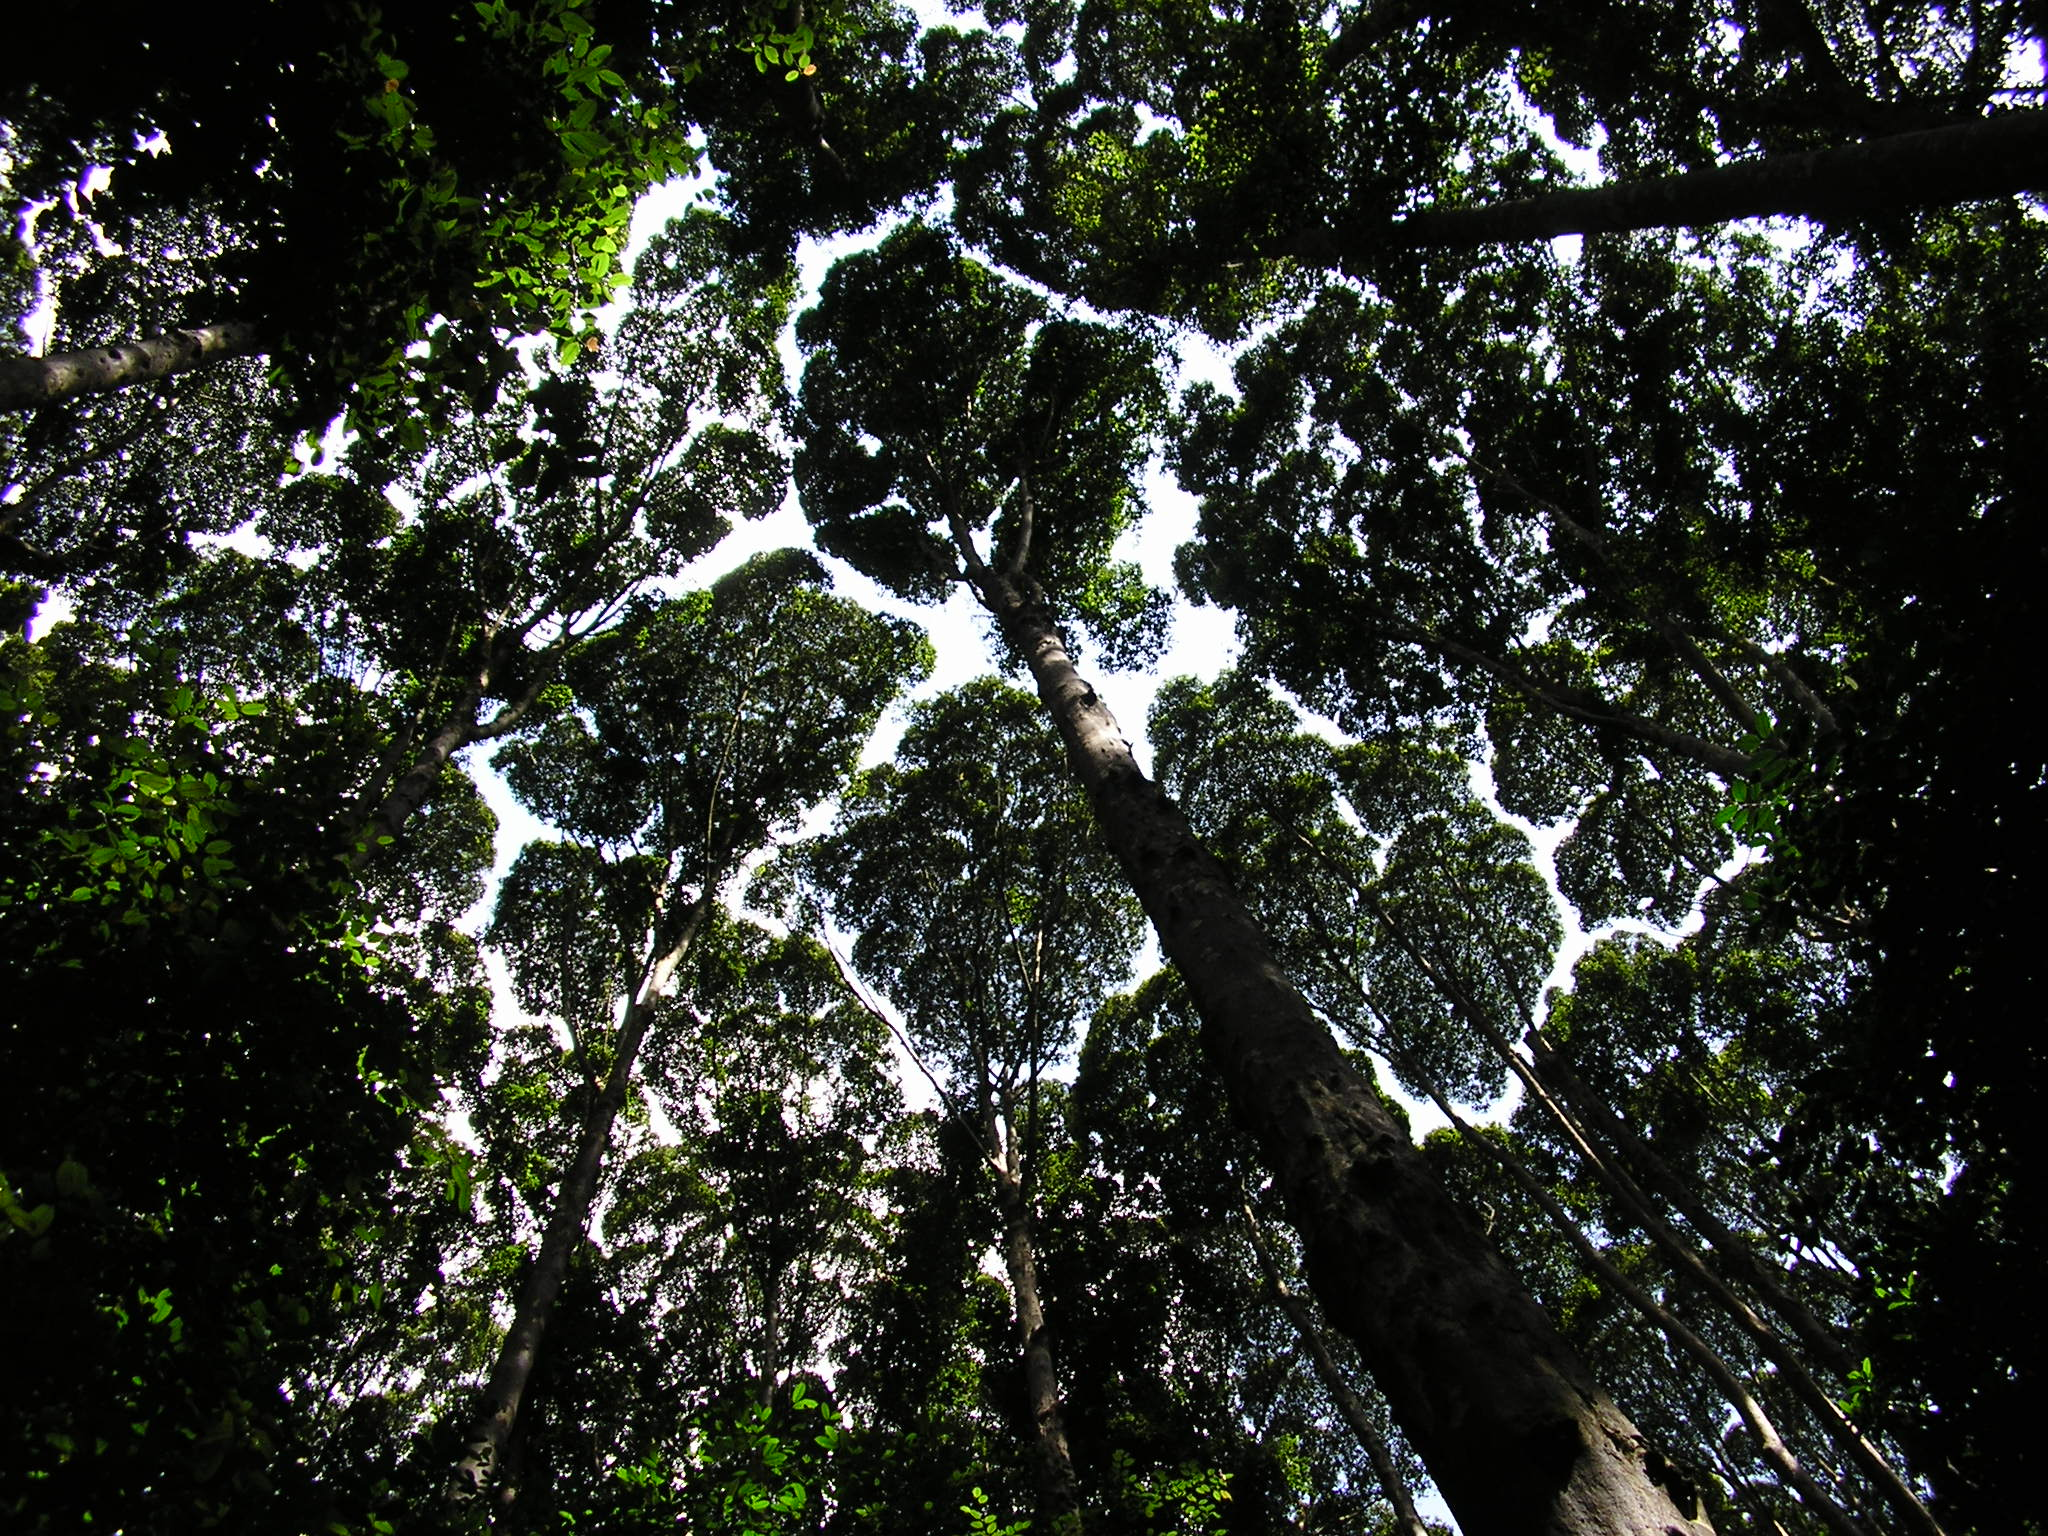
\includegraphics[height=\paperheight,width=\paperwidth]{./Figures/Canopy.png}}
  \setbeamertemplate{navigation symbols}{}

  \begin{frame}[plain]
    \begin{block}{}
      \begin{center}
        \ldots~Thank you for attention~\ldots
      \end{center}
    \end{block}
  \end{frame}
}

\end{document}
